\begin{frame}{Opis problemu}
    \begin{block}{Podział zbioru}
        Mamy dany zbiór n wartości rzeczywistych $\{a_1, \cdots, a_n\}$. Czy da się podzielić zbiór na dwa podzbiory $A_1$ i $A_2$ takie, żeby suma $A_1$ równała się subie wartości $A_2$? (Problem NP-zupełny)
    \end{block}

    \begin{block}{Podział zbioru (wersja optymalizacyjna)}
        Znaleźć podział dający najmniejszy moduł róznic sum.    
    \end{block}

\end{frame}

\begin{frame}{Opis problemu}
    \begin{figure}
        \centering
        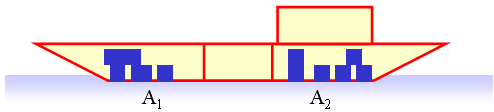
\includegraphics[width=8cm]{obrazki/statek.png}
        \caption{Problem podziału zbioru na przykładzie statku towarowego}
    \end{figure}
    \begin{block}{Podział zbioru (opis praktyczny)}
        Rozmieścić towar (kontenery o róznej masie) w ładowni dziobowej i rufowej tak, by statek był w równowadze.
    \end{block}
\end{frame}

\begin{frame}{Reprezentacja danych i rozwiązań}
    \begin{block}{Dane problemu}
        Ciąg liczb rzeczywistych $\{a_i\}_n$ długości $n$ reprezentujących wagi poszczególnych towarów.
    \end{block}

    \begin{block}{Rozwiązanie problemu}
        Wektor binarny $\{x_i\}_n$ ($x_i \in \{0, 1\}$) długości $n$ przyporządkowujący i'ty towar do zbioru $x_i$.
    \end{block}

    \begin{block}{Funkcja celu}
        \begin{equation}
            f(x) = \left| \sum\limits_{i=1}^{n} a_i \cdot (2 \cdot x_i - 1) \right| = \left| \sum\limits_{x \in A_1} x - \sum\limits_{y \in A_2} y \right|
        \end{equation}
    \end{block}
\end{frame}

\begin{frame}{Planowane rozwiązanie}
    \begin{block}{Planowane rozwiązanie}
 
    \end{block}
    % http://edu.pjwstk.edu.pl/wyklady/nai/scb/wyklad7/w7.htm
\end{frame}
